
\graphicspath{ {SectionInstallationGuide/} }

\section{Installation Guide}
\label{sec:installation_guide}

This section guides the reader through the installation of the necessary software in order to start using the SML World. It will first focus on the installation of Python and afterwards on the additional Python libraries required for the SML World to run.

The instructions are targeted for a Windows system. The SML World is also able to run in Unix systems, as long as Python and the required libraries are installed. A guide for installing in Unix systems is not provided, as we assume that a Unix user should be able to easily understand the Windows Installation procedure, and will have not trouble in adapting it to his own system.

\subsection{Python Installation and Setup}

The SML World was developed using Python 2.7. In order to run Python programs you need to install the software available at \url{https://www.python.org/downloads/}. Select Python version $2.7.x$ as shown in figure \ref{fig:python_install_download}

\begin{figure}[h!]
  \centering
    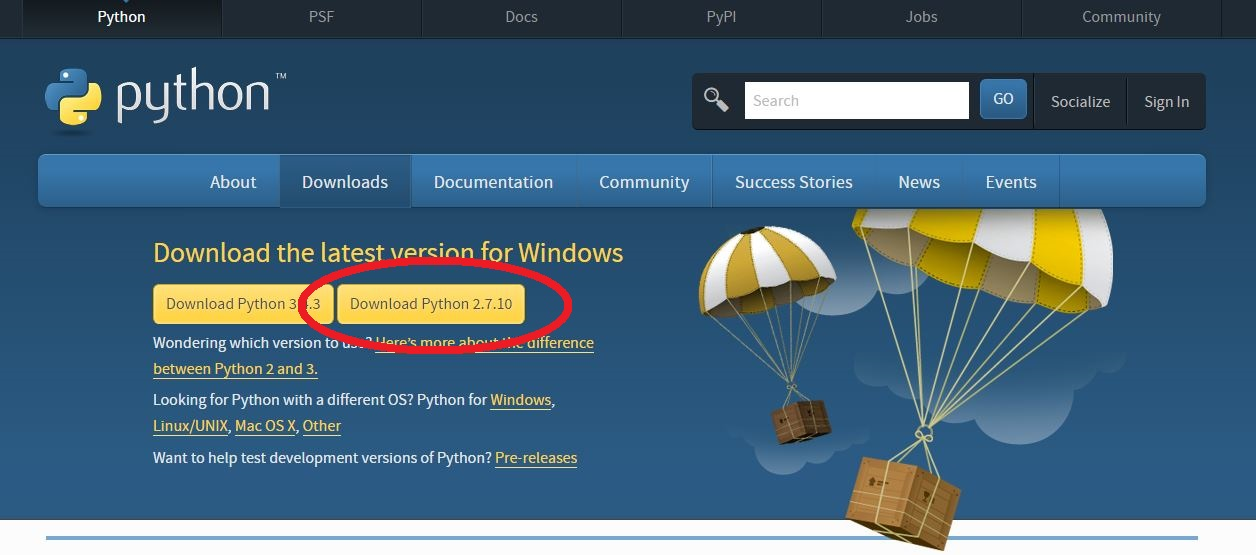
\includegraphics[width=0.6\textwidth]{python_install_1}
    \caption{Downloading Python $2.7.x$ \label{fig:python_install_download} }
\end{figure}


Right click the downloaded file and select Install. Follow the installation instructions, and when you arrive at the window shown in figure \ref{fig:python_install_option_add_path}, select “Will be installed on local drive” for the \textit{Add python.exe to Path} option.

\begin{figure}[h!]
  \centering
    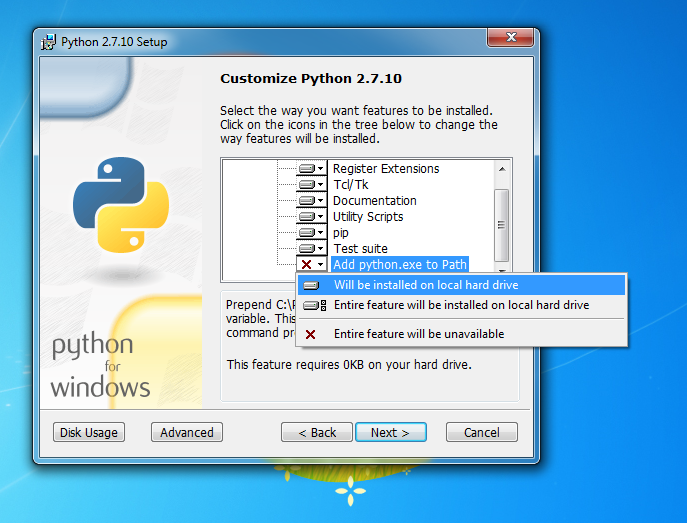
\includegraphics[width=0.6\textwidth]{python_install_3}
    \caption{Adding Python to the System Path \label{fig:python_install_option_add_path} }
\end{figure}

Press next, and the installation will continue, and eventually finish. To test if Python was successfully installed, simply open a terminal (to do so, open the Start Menu, and write \texttt{cmd} in the search bar, and click \texttt{cmd.exe}, figure \ref{fig:python_install_open_terminal}), and enter the command \texttt{python}. The result should be the one shown in figure \ref{fig:python_install_python_command}. If it is, you can jump to section \ref{subsec:installing_python_libraries}  and start installing the Python libraries.

If you cannot replicate the result seen in the figure, and instead get the message \texttt{'python' is not recognized as an internal or external command, operable program or batch file}, then go to section \ref{subsec:adding_python_to_environment_path}.

\begin{figure}[h!]
  \centering
    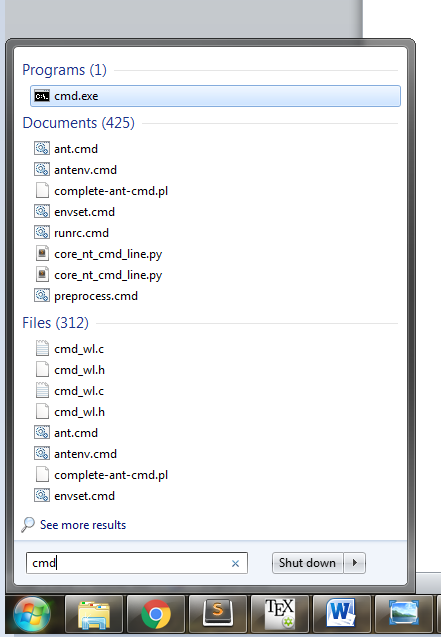
\includegraphics[width=0.6\textwidth]{python_install_opening_terminal}
    \caption{Opening a terminal \label{fig:python_install_open_terminal} }
\end{figure}


\begin{figure}[h!]
  \centering
    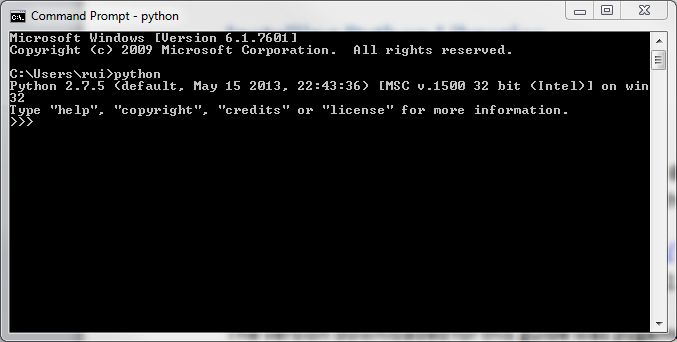
\includegraphics[width=0.9\textwidth]{python_install_terminal_python_command}
    \caption{Running the \texttt{python} command \label{fig:python_install_python_command} }
\end{figure}

\subsection{Manually Adding Python To Environment Path}
\label{subsec:adding_python_to_environment_path}

If you installed Python, but cannot run it, then the reason might be that Python was not added to the windows Path variable. This Path variable, contains information about the location of programs, so that they can be called/run from the command line.

The first thing to do is to find where your Python installation folder is located. If you followed the default installation steps, then your Python folder should be at \texttt{C:\\Python27}, as seen in figure \ref{fig:python_install_python_folder}. If it is not there, try to locate it in other possible folders (suggestions: \texttt{ProgramFiles}, \texttt{ProgramFiles (x86)}).

\begin{figure}[h!]
  \centering
    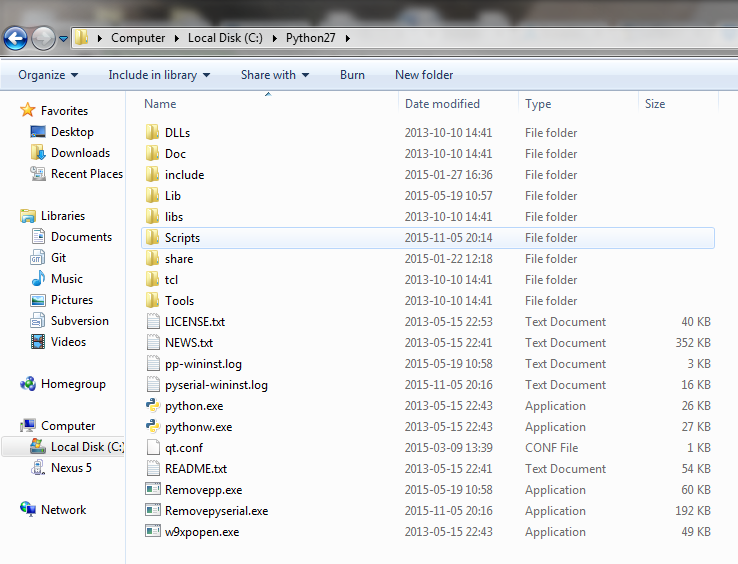
\includegraphics[width=0.9\textwidth]{python_install_python_folder}
    \caption{The python installation folder \label{fig:python_install_python_folder} }
\end{figure}

Now that you located the folder where \texttt{python.exe} is, you need to add it to the Windows Path Variable. To do so, open the Windows Menu, and type \texttt{var} in the search bar, then select \texttt{Edit the system environment variables}, as seen in figure \ref{fig:python_install_opening_environment_variables}.


\begin{figure}[h!]
  \centering
    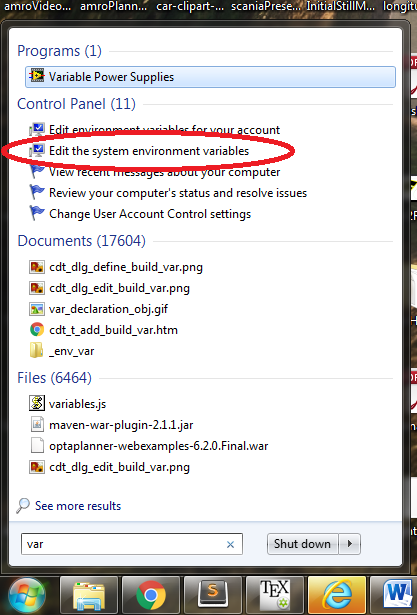
\includegraphics[width=0.6\textwidth]{python_install_4}
    \caption{Opening the System Environment Variables \label{fig:python_install_opening_environment_variables} }
\end{figure}

The \texttt{System Properties} window will open, press \texttt{Environment Variables...}, in the new window, find the \texttt{path} variable, and click \texttt{Edit...} (in case the \texttt{path} variable does not exist you will need to create it by pressing \texttt{New...}). A new window appears, now you simply have to add the folder path of the Python folder, simply add \texttt{C:\\Python27} (or another directory where you installed Python), with a preceding semicolon to separate it from other paths that might already be there. Figure \ref{fig:python_install_adding_to_the_path_variable} shows this process. In this case the Python location is between two other locations, so it has a semicolon before and another after.

\begin{figure}[h!]
  \centering
    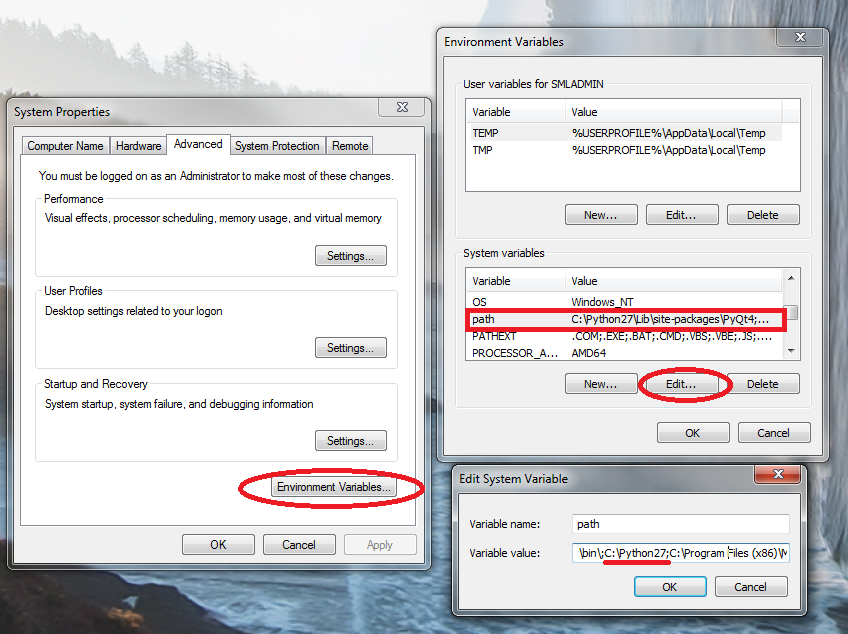
\includegraphics[width=0.9\textwidth]{python_install_6_highlighted}
    \caption{Editing the Path Variable \label{fig:python_install_adding_to_the_path_variable} }
\end{figure}

Close the terminal and reopen it (necessary so that it uses the new System Variable Path). Type Python, you should now be able to see figure \ref{fig:python_install_python_command}.

\subsection{Installing Additional Python Libraries}
\label{subsec:installing_python_libraries}

Python libraries are modules that provide python with specific high level programming commands, that allow the user to develop code with less effort and bigger productivity.

\subsubsection{Installing pygame}

Pygame is a library that allows the programmer to develop nice graphical visualisations with ease. This library is used by the Visualisation and Road Modules in order to display and generate the SML World environment.

Pygame can be found in \url{http://www.pygame.org/}. Simply go to the Downloads page, and select the correct pygame version for your Python version (2.7).
The version downloaded for this guide was \texttt{pygame-1.9.1.win32-py2.7.msi} (3.1MB). Simply run the file, and install using all the default installation settings.

\subsubsection{Installing NumPy}

The NumPy library provides the developer with mathematical tools that can be useful in a large number of situations.

To install it you will need to access \url{http://www.lfd.uci.edu/~gohlke/pythonlibs/}, 

and go to the NumPy section
 \url{http://www.lfd.uci.edu/~gohlke/pythonlibs/\#numpy}.
 You should download the .whl file that suits your python and computer version, in this tutorial \texttt{numpy-1.9.2+mkl-cp27-none-win32.whl} is used. The \texttt{27} in the filename indicates that this is numpy for the Python 2.7 version.

Open the terminal in the folder where the file we just downloaded is located. You can do it by simply pressing \texttt{SHIFT+RIGHT CLICK} and then pressing Open command window here, see figure \ref{fig:numpy_install_open_terminal}.

\begin{figure}[h!]
  \centering
    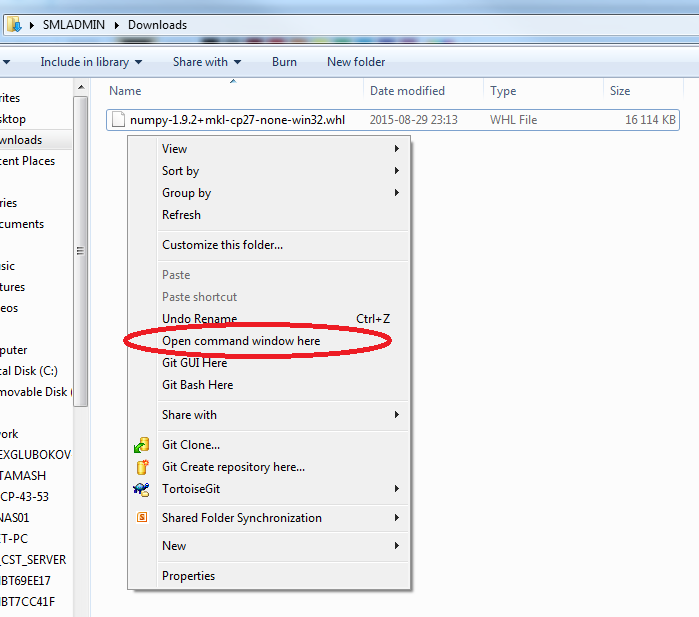
\includegraphics[width=0.9\textwidth]{numpy_install_open_terminal_highlighted}
    \caption{Opening the terminal in a folder location \label{fig:numpy_install_open_terminal} }
\end{figure}

In the terminal that opens run the command \texttt{pip install \"numpy-1.9.2+mkl-cp27-none-win32.whl\"}. This will call Python's \texttt{pip} program that allows for an easy installation of Python libraries. 

\begin{figure}[h!]
  \centering
    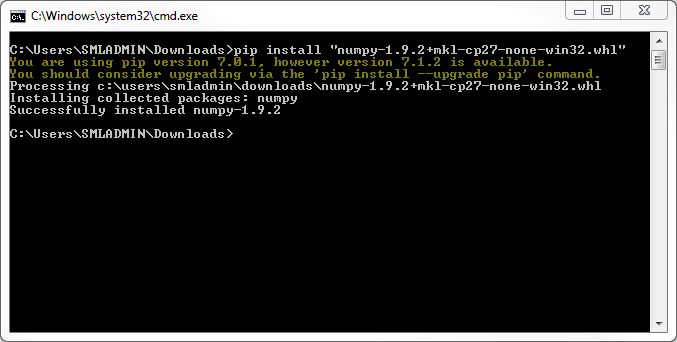
\includegraphics[width=0.9\textwidth]{numpy_install_success}
    \caption{Successful installation of NumPy using \texttt{pip install} \label{fig:numpy_install_success} }
\end{figure}

If you get the error \texttt{'pip' is not recognized as an internal or external command, operable program or batch file}, then you need to add \texttt{pip} to the Environment Variable Path (see section \ref{subsubsec:adding_pip_to_path}).

If the installation was sucessful, like shown in image \ref{fig:numpy_install_success}, then go to section \ref{subsubsec:installing_shapely}.

\subsubsection{Adding Pip to Environment Path}
\label{subsubsec:adding_pip_to_path}

The \texttt{pip} program is included in the current versions of the Python installer. To check that you have it in your system simply go to the Python installtion folder, and check the \texttt{Scripts} folder in it, it should contain an executable \texttt{pip.exe}. To be able to run \texttt{pip install} from the command line you need to add this folder to the System Variable Path. The process is the same as the one explained in section \ref{subsec:adding_python_to_environment_path}, however instead of adding the Python folder location we add the Python\\Scripts folder location, as seen in figure \ref{fig:pip_install_environment_variable}.

\begin{figure}[h!]
  \centering
    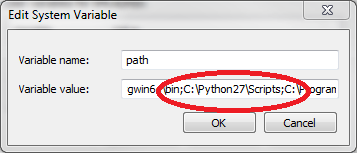
\includegraphics[width=0.7\textwidth]{pip_install_environment_variable_highlighted}
    \caption{Adding \texttt{pip} to variable Path \label{fig:pip_install_environment_variable} }
\end{figure}

To test that you successfully added \texttt{pip} to the System Variable Path simply close and reopen the terminal, and type the command \texttt{pip install}. You should see have the same result as figure \ref{fig:pip_install_test}.

\begin{figure}[h!]
  \centering
    \includegraphics[width=0.9\textwidth]{pip_install_test}
    \caption{Successful installation of \texttt{pip} \label{fig:pip_install_test} } 
\end{figure}

\subsubsection{Choosing the correct .whl File}
\label{subsubsec:choosin_whl_file}

\subsubsection{Installing Shapely}
\label{subsubsec:installing_shapely}

Shapely is currently only being used by the Blockly Module. You only need to install it in case you pretend to run the SML School code. Shapely is a module that allows for simple handling and operation of geometric objects.

Similarly to NumPy, it can be downloaded and installed using \texttt{pip install}. First download Shapely from \url{http://www.lfd.uci.edu/~gohlke/pythonlibs/#shapely}. In this guide the downloaded file was \texttt{Shapely-1.5.12-cp27-none-win32.whl}. The installation process is identical to NumPy's installation. 
